% !TEX program = xelatex

\documentclass{ctexart}
\usepackage{ctex}
\usepackage[a4paper, left=20mm, right=20mm, top=30mm, bottom=30mm]{geometry}
\usepackage{graphicx}
\graphicspath{ {./images/} }
\usepackage{hyperref}
\hypersetup{
  colorlinks=true,
  linkcolor=black
}
\usepackage{xcolor}
\usepackage{listings}

% listings宏包配置,引用自:
% 怎么在 LaTeX 中排版 Python 代码? - 孟晨的回答 - 知乎
% https://www.zhihu.com/question/65508676/answer/232267619
\lstdefinestyle{lfonts}{
  basicstyle   = \footnotesize\ttfamily,
  stringstyle  = \color{purple},
  keywordstyle = \color{blue!60!black}\bfseries,
  commentstyle = \color{olive}\scshape,
}
\lstdefinestyle{lnumbers}{
  numbers     = left,
  numberstyle = \tiny,
  numbersep   = 1em,
  firstnumber = 1,
  stepnumber  = 1,
}
\lstdefinestyle{llayout}{
  breaklines       = true,
  tabsize          = 2,
  columns          = flexible,
}
\lstdefinestyle{lgeometry}{
  xleftmargin      = 20pt,
  xrightmargin     = 0pt,
  frame            = tb,
  framesep         = \fboxsep,
  framexleftmargin = 20pt,
}
\lstdefinestyle{lgeneral}{
  style = lfonts,
  style = lnumbers,
  style = llayout,
  style = lgeometry,
}
\lstdefinestyle{python}{
    language = {Python},
    style    = lgeneral,
}

\author{
	冯国蕴 \and 林欣煜 \and 马詠汛 \and 谢金宏
}
\title{使用细胞自动机模拟简单生态系统}
\date{2019年12月21日}

\begin{document}

\maketitle

\begin{abstract}
在本次课题中,我们小组使用Python语言实现了基本的细胞自动机。并在已有的细胞自动机的规则基础上进行扩展,尝试对具有氧气、生产者和消费者三要素的生态系统进行模拟。
\end{abstract}

\tableofcontents

\section{细胞自动机与康威生命游戏}

细胞自动机\footnote{Cellular automaton \url{https://en.wikipedia.org/wiki/Cellular_automaton}}最早由冯·诺依曼在1950年代为模拟生物细胞的自我复制而提出,起初未受到科学界的广泛关注。后因约翰·何顿·康威设计了生命游戏\footnote{Conway's Game of Life \url{https://en.wikipedia.org/wiki/Conway's_Game_of_Life}}而闻名于世。本节将简要介绍细胞自动机与康威生命游戏。

\subsection{细胞自动机}

我们可以在二维的格状棋盘上实现细胞自动机。在这个二维的空间上,棋盘中每个格子内细胞的状态是有限的,细胞下一时刻的状态由该细胞的邻居在当前的时刻的状态决定。棋盘内的所有细胞遵守相同的演化规则。

即一个细胞自动机一般具有以下特点:

\begin{itemize}
  \item \textbf{平行计算 }每个细胞个体的状态都同步地进行改变。
  \item \textbf{局部性 }细胞的状态只受相邻的细胞的影响。
  \item \textbf{一致性 }所有的细胞受到相同的规则约束。
\end{itemize}

\subsection{康威生命游戏}

康威生命游戏符合细胞自动机的特点,其规则定义如下:

\begin{itemize}
  \item 每种细胞有“存活”和“死亡”两种状态。
  \item 当细胞周围的存活细胞数量等于3个时,细胞变为存活状态。
  \item 当细胞周围的存活细胞数量少于等于1个或大于等于4个时,细胞变为死亡状态。(模拟细胞过于孤独或环境过于拥挤。)
  \item 其他情况下细胞状态不变。
\end{itemize}

我们小组使用Python实现了经典的康威生命游戏(\underline{1.basic.py})。程序先随机地给定棋盘内细胞初始状态,然后按照康威生命游戏规则演化指定的代数,给出最终的结果。

\begin{figure}[h]
  \centering
  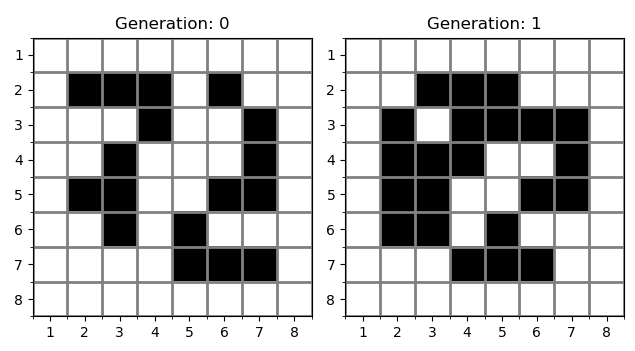
\includegraphics[scale=0.75]{1.png}
  \caption{按康威生命游戏规则进行一次迭代}
  \label{fig:1}
\end{figure}

图\ref{fig:1}是随机产生初始状态后按康威规则演化一代的结果。图中黑色块表示活细胞,白色块表示空位或死细胞。

\subsection{镜像边界}

细胞自动机理论上具有无穷大的“棋盘”作为细胞演化的空间,但计算机的内存空间是有限的,故无限大的棋盘不能实现,实际运行中的棋盘往往是规模为$n$的矩形棋盘。有限的空间就存在边界问题,边界上的细胞因此需要特殊处理。

在\underline{1.basic.py}中,边界上的细胞不参与演化,它们总是保持死细胞的状态。这是处理边界问题的一种方法,即边界上的细胞取得定值,在演化过程中保持不变。

另一种处理边界细胞问题的方法是在\underline{1.basic-mirror-edge.py}中实现的镜像边界。如图\ref{fig:2}所示,编号为1的细胞,它的左上角邻居、左邻居和右邻居分别被镜像地设置为9号、3号和7号细胞。

\begin{figure}[h]
  \centering
  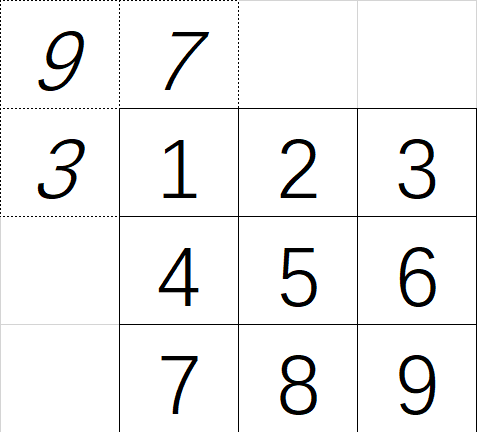
\includegraphics[scale=0.75]{2.png}
  \caption{镜像边界的一个实例}
  \label{fig:2}
\end{figure}

一般地,对于采用镜像边界的$SIZE$大小的棋盘,格点位置为$(i, j)$的细胞,它的邻居可以通过如下程序遍历:

\begin{lstlisting}[style = python]
for i, j in CELLS:
  for dx in range(-1, 2):
    for dy in range(-1, 2):
      neighbor = board.iat[(i + dx + SIZE) % SIZE, (j + dy + SIZE) % SIZE]
\end{lstlisting}

如无特殊说明,本文后续的模型均采用镜像边界的处理方法。

\subsection{康威生命游戏的几个经典图案}

我们在程序中实现了康威生命游戏的几个经典图像。

\section{氧气扩散模型}

为了模拟生态系统中的一些问题。

\section{光照和生产者模型}

\section{消费者模型}

\section{模拟生态系统}

\section{结语}

\end{document}
